\documentclass[12pt,a4paper]{article}
\usepackage[utf8]{inputenc}
\usepackage[german]{babel}
\usepackage[T1]{fontenc}
\usepackage{amsmath}
\usepackage{amsfonts}
\usepackage{amssymb}
\usepackage{graphicx}
\usepackage{siunitx}
\usepackage[left=2cm,right=2cm,top=2cm,bottom=2cm]{geometry}
\author{Tim}

\begin{document}
\setlength{\parindent}{0pt} 
\begin{center}
{\LARGE Versuchsprotokoll}\\
\begin{large}
zum Grundpraktikum Physik Teil II\\[0.4cm]
an der RWTH Aachen\\
I. Physikalisches Institut B\\[4.5cm]
\Large\textbf{\textsl{Optik II}}\\[4cm]
\normalsize\textit{vorgelegt\\von}\\[0.4cm]
\large{Moritz Berger\\Tim Herbermann\\Gerald Kolter\\Sebastian Siebert}\\[1cm]
\large \textit{Gruppe A07} \\ [3cm]
\large \textbf{Sommersemester 2017}
\end{large}
\end{center}
\newpage

\tableofcontents
\newpage

\section{Grundlagen}

Im folgenden Versuch soll mithilfe eines Michelson-Interferometers die Wellenlänge eines Lasers bestimmt werden. Anschließend soll die Druckabhängigkeit des Brechungsindex von Luft untersucht werden. Als letztes wird der Brechungsindex von $\text{CO}_2$ bestimmt.\\
\\
Grundlage des Versuches ist  die Interferenz eines kohärenten Wellenzuges mit sich selbst durch Amlitudenaufspaltung. Die dadurch entstehenden Teilstrahlen durchlaufen eine unterschiedliche Strecke, bis sie wieder vereinigt werden. Dadurch besitzen sie eine feste Phasenbeziehung zueinander und somit eine konstante Interferenz.\\
Beim Michelson-Interferometer wird ein leicht diverenter Strahl verwendet. Dadurch gibt es für unterschiedliche Divergenzwinkel $\theta$ andere Phasenverschiebungen, da die Strecke mit $\cos(\theta)$ modifiziert wird. Für den Streckenunterschied gilt dann:
\begin{equation}
\delta = \dfrac{2\pi}{\lambda} \cdot 2d \cos(\theta)
\end{equation}
Betrachtet man Interferenzmaxima muss $\delta = 2\pi m$, $m=0,1,2,...$, gelten und damit:
\begin{equation}
2d \cos(\theta) = m\lambda
\end{equation}


\section{Aufbau und Durchführung}
\begin{figure}
\centering
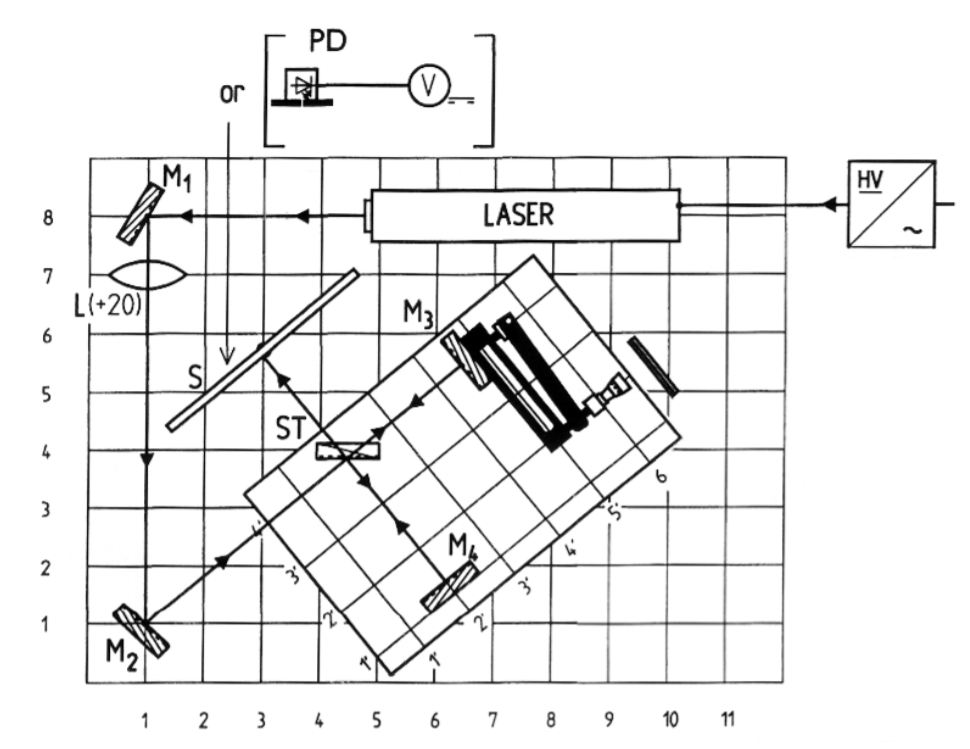
\includegraphics[scale=0.6]{Bilder/Aufbau}
\caption{Aufbau eines Michelson-Interferometers}
\label{fig:Aufbau}
\end{figure}


\section{Auswertung}

\subsection{Kalibration}

\subsection{Bestimmung der Wellenlänge}

\subsection{Druckabhängigkeit des Brechungsindex}

\subsection{Brechungsindex von Kohlenstoffdioxid}

\section{Fazit}

\end{document}
